% Standalone render of generated/table_buy_signal.tex
% Build: pdflatex -interaction=nonstopmode buy_signal_standalone.tex
\documentclass{article}
\usepackage[landscape,margin=0.4in]{geometry}
\usepackage{booktabs}
\usepackage{amsmath}
\usepackage{graphicx}
\pagestyle{empty}
\begin{document}
\begin{center}
\textbf{0DTE 15:30--16:00 nearest-OTM package: how often the signal is right, and by how much, 866 common days}\\[1.5ex]
% AUTO-GENERATED by writeup/make_buy_signal_tex.py -- do not edit.
% Source: results/atm_straddle_0dte_1530/buy_signal_reading.csv and daily_blk2.parquet
\begingroup\small\setlength{\tabcolsep}{5pt}
\begin{tabular}{lrrrrrr}
\toprule
& $n$ & hit rate & avg.\ win & avg.\ loss & mean/day & $P(R=-1)$ \\
\midrule
\multicolumn{7}{l}{\emph{Buy days ($s_t>0$): the long package's return $R$}} \\
baseline (HAR + calendar OLS) & 286 & 0.399 & +1.267 & -0.703 & +0.082 & 0.231 \\
block-diagonal ridge & 346 & 0.408 & +1.284 & -0.713 & +0.100 & 0.228 \\
block-diagonal ridge, no FOMC columns & 355 & 0.406 & +1.276 & -0.716 & +0.092 & 0.228 \\
LightGBM & 290 & 0.393 & +1.407 & -0.693 & +0.133 & 0.224 \\
XGBoost & 279 & 0.398 & +1.406 & -0.693 & +0.142 & 0.222 \\
lasso (causally tuned) & 321 & 0.408 & +1.311 & -0.709 & +0.115 & 0.215 \\
lasso ($\alpha=10^{-4}$) & 358 & 0.405 & +1.335 & -0.721 & +0.112 & 0.232 \\
elastic net (causally tuned) & 307 & 0.397 & +1.289 & -0.714 & +0.082 & 0.225 \\
\emph{base rate: long the package every day} & 866 & 0.381 & +1.072 & -0.684 & -0.014 & 0.223 \\
\midrule
\multicolumn{7}{l}{\emph{Sell days ($s_t\le 0$): the short package's return $-R$}} \\
baseline (HAR + calendar OLS) & 580 & 0.626 & +0.676 & -0.965 & +0.062 & 0.219 \\
block-diagonal ridge & 520 & 0.635 & +0.667 & -0.910 & +0.091 & 0.219 \\
block-diagonal ridge, no FOMC columns & 511 & 0.634 & +0.665 & -0.910 & +0.089 & 0.219 \\
LightGBM & 576 & 0.623 & +0.681 & -0.892 & +0.088 & 0.222 \\
XGBoost & 587 & 0.625 & +0.681 & -0.899 & +0.089 & 0.223 \\
lasso (causally tuned) & 545 & 0.633 & +0.672 & -0.911 & +0.091 & 0.228 \\
lasso ($\alpha=10^{-4}$) & 508 & 0.634 & +0.661 & -0.862 & +0.103 & 0.217 \\
elastic net (causally tuned) & 559 & 0.626 & +0.670 & -0.941 & +0.067 & 0.222 \\
\emph{base rate: short the package every day} & 866 & 0.618 & +0.685 & -1.069 & +0.014 & 0.223 \\
\bottomrule
\end{tabular}
\endgroup

\end{center}
\vspace{1ex}
\begin{center}
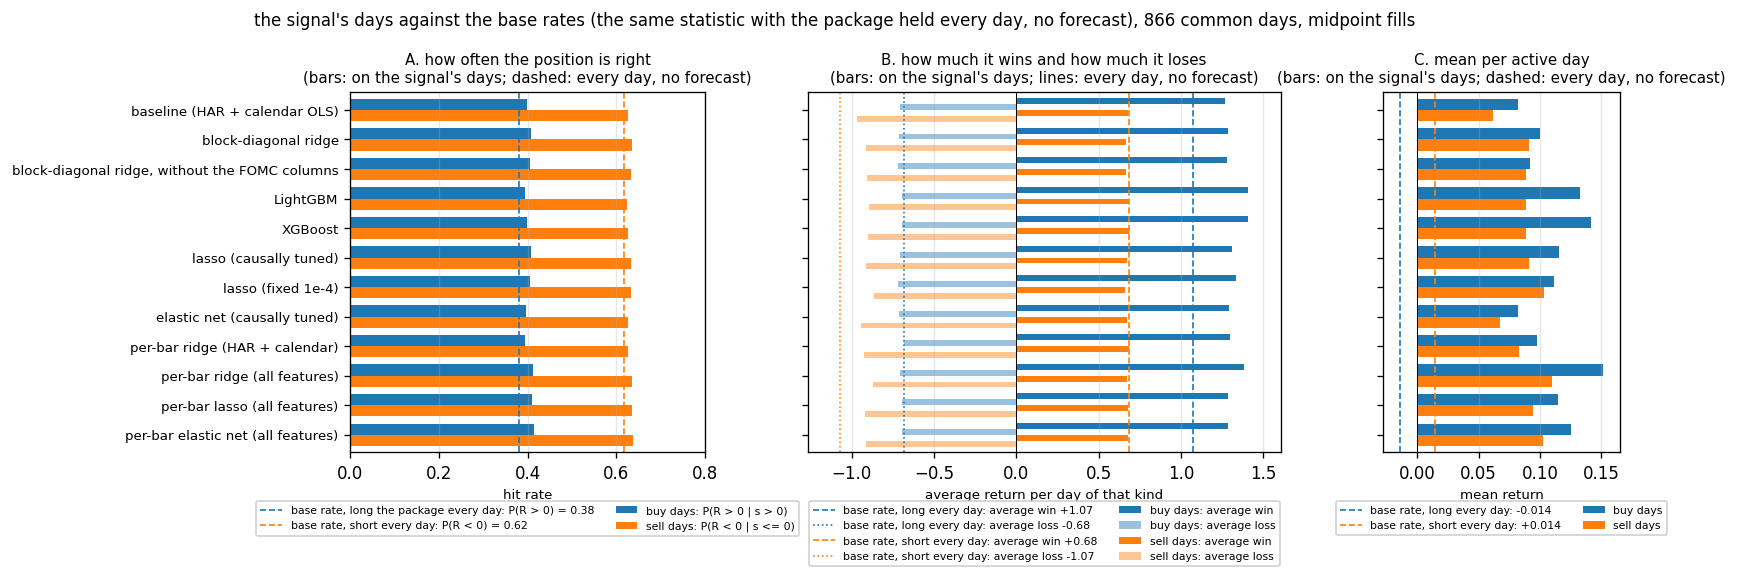
\includegraphics[width=0.78\textwidth]{../results/atm_straddle_0dte_1530/buy_signal_hitrate.png}
\end{center}
\vspace{1ex}
\noindent\small A hit on a buy day is $R>0$; on a sell day it is $R<0$. The average win and loss are the
conditional means of the position's return, $R$ on buy days and $-R$ on sell days, on its winning and
losing days; mean/day is the position's mean return per active day; $P(R=-1)$ is the share of days the
package expires worthless. The base-rate rows are the same statistics over all 866 days with the package
held every day and no forecast: long for the buy panel, short for the sell panel. Mid fill; returns in
units of the entry premium. In the figure, bars are the signal's days and the dashed lines are the base rates.
\end{document}
